%%
%% This is file `sample-sigconf.tex',
%% generated with the docstrip utility.
%%
%% The original source files were:
%%
%% samples.dtx  (with options: `sigconf')
%% 
%% IMPORTANT NOTICE:
%% 
%% For the copyright see the source file.
%% 
%% Any modified versions of this file must be renamed
%% with new filenames distinct from sample-sigconf.tex.
%% 
%% For distribution of the original source see the terms
%% for copying and modification in the file samples.dtx.
%% 
%% This generated file may be distributed as long as the
%% original source files, as listed above, are part of the
%% same distribution. (The sources need not necessarily be
%% in the same archive or directory.)
%%
%%
%% Commands for TeXCount
%TC:macro \cite [option:text,text]
%TC:macro \citep [option:text,text]
%TC:macro \citet [option:text,text]
%TC:envir table 0 1
%TC:envir table* 0 1
%TC:envir tabular [ignore] word
%TC:envir displaymath 0 word
%TC:envir math 0 word
%TC:envir comment 0 0
%%
%%
%% The first command in your LaTeX source must be the \documentclass command.
\documentclass[sigplan,10pt]{acmart}

\usepackage{fontawesome}
% To enable T_ without mathmode
\usepackage{xspace}

% custom packages
% \usepackage[textsize=scriptsize]{todonotes}
% \presetkeys{todonotes}{fancyline}{}
%TODO jo: are we sure we can change this as per the CFP? Usually the margins are set in the CFP and messing with them, increasing space, may lead to desk-reject!
%TODO jt: don't worry, this only affects the behaviour of todonotes, can be
%removed before submission without layout explosions
%\setlength{\marginparwidth}{1.8cm}
%\setlength{\marginparsep}{3pt}
\usepackage{lipsum}

% \newcommand{\jo}[1]{\todo[color=yellow]{\textbf{Jo:} #1}}
% \newcommand{\jt}[1]{\todo{\textbf{JT:} #1}}
% \newcommand{\fritz}[1]{\todo[color=blue!20]{\textbf{Fritz:} #1}}
% \newcommand{\gianluca}[1]{\todo[color=red!20]{\textbf{Gianluca:} #1}}
% \newcommand{\christoph}[1]{\todo[color=orange!20]{\textbf{Christoph:} #1}}

\usepackage[capitalize]{cleveref}
\usepackage{enumitem}

\usepackage{tabularx, multirow}
\usepackage{adjustbox}
\usepackage{wasysym}
\usepackage{pifont}
\newcommand{\cmark}{\ding{51}}%
\newcommand{\xmark}{\ding{55}}%
\usepackage{gensymb}
\usepackage{fontawesome}


% No idea whether you folks will also write SMM or other so I'll just put SMM in acro
\usepackage[nolist,nohyperlinks]{acronym}

\acrodef{DRM}{digital rights management}
\acrodef{JWT}{JSON web token}
\acrodef{ME}{management engine}
\acrodef{MSR}{model-specific register}
\acrodef{PSW}{platform software}
\acrodef{SDK}{software development kit}
\acrodef{SMM}{system management mode}
\acrodef{SNP}{secure nested paging}
\acrodef{TD}{trusted domain}
\acrodef{TEE}{trusted execution environment}
\acrodef{TOTP}{time-based one-time password}
\acrodef{TPM}{trusted platform module}
\acrodef{TSC}{timestamp counter}
\acrodef{UTC}{coordinated universal time}

% jo: we can decide on a uniform style to format x86 instructions here
%\newcommand{\inst}[1]{\texttt{\uppercase{#1}}}
\newcommand{\inst}[1]{\texttt{\lowercase{#1}}}
%\newcommand{\inst}[1]{\texttt{\textsc{\lowercase{#1}}}}


%%
%% \BibTeX command to typeset BibTeX logo in the docs
\AtBeginDocument{%
  \providecommand\BibTeX{{%
    Bib\TeX}}}

%% Rights management information.  This information is sent to you
%% when you complete the rights form.  These commands have SAMPLE
%% values in them; it is your responsibility as an author to replace
%% the commands and values with those provided to you when you
%% complete the rights form.
\acmYear{2023}\copyrightyear{2023}
\setcopyright{acmlicensed}
\acmConference[SysTEX '23]{6th Workshop on System Software for Trusted Execution}{May 8, 2023}{Rome, Italy}
\acmBooktitle{6th Workshop on System Software for Trusted Execution (SysTEX '23), May 8, 2023, Rome, Italy}
\acmPrice{15.00}
\acmDOI{10.1145/3578359.3593038}
\acmISBN{979-8-4007-0087-3/23/05}


%%
%% Submission ID.
%% Use this when submitting an article to a sponsored event. You'll
%% receive a unique submission ID from the organizers
%% of the event, and this ID should be used as the parameter to this command.
%%\acmSubmissionID{123-A56-BU3}

%%
%% For managing citations, it is recommended to use bibliography
%% files in BibTeX format.
%%
%% You can then either use BibTeX with the ACM-Reference-Format style,
%% or BibLaTeX with the acmnumeric or acmauthoryear sytles, that include
%% support for advanced citation of software artefact from the
%% biblatex-software package, also separately available on CTAN.
%%
%% Look at the sample-*-biblatex.tex files for templates showcasing
%% the biblatex styles.
%%

%%
%% The majority of ACM publications use numbered citations and
%% references.  The command \citestyle{authoryear} switches to the
%% "author year" style.
%%
%% If you are preparing content for an event
%% sponsored by ACM SIGGRAPH, you must use the "author year" style of
%% citations and references.
%% Uncommenting
%% the next command will enable that style.
%%\citestyle{acmauthoryear}


%%
%% end of the preamble, start of the body of the document source.
\begin{document}

%%
%% The "title" command has an optional parameter,
%% allowing the author to define a "short title" to be used in page headers.
%title{An Analysis of Trusting Time with Trusted Computing Architectures}
%\title{No time for TEE:\\How TEEs Struggle With Providing Trusted Time}
%\title{TEE Time: On the Challenges of Providing Temporal Guarantees in Untrusted Environments}
\title{About Time: On the Challenges of Temporal Guarantees in Untrusted Environments}

%%
%% The "author" command and its associated commands are used to define
%% the authors and their affiliations.
%% Of note is the shared affiliation of the first two authors, and the
%% "authornote" and "authornotemark" commands
%% used to denote shared contribution to the research.
% \author{Gianluca Scopelliti}
% \authornote{Both authors contributed equally to this research.}
% \email{trovato@corporation.com}
% \orcid{1234-5678-9012}
% \author{G.K.M. Tobin}
% \authornotemark[1]
% \email{webmaster@marysville-ohio.com}
% \affiliation{%
%   \institution{Institute for Clarity in Documentation}
%   \streetaddress{P.O. Box 1212}
%   \city{Dublin}
%   \state{Ohio}
%   \country{USA}
%   \postcode{43017-6221}
% }


\newcommand{\affiliationkul}{
  \affiliation{
  \department{imec-DistriNet, KU Leuven, Belgium}
  \institution{}
%   \city{Leuven}
  \country{}
%   \postcode{3001}
  }
}
\newcommand{\affiliationeab}{
  \affiliation{
  \department{Ericsson Security Research, Sweden}
  \city{}
  \country{}
  }
}
\newcommand{\affiliationulb}{
  \affiliation{
%  \department{Ecole Polytechnique, BEAMS \& Cybersecurity Research Center, Universit\'e Libre de Bruxelles, Belgium}
  \department{Universit\'e Libre de Bruxelles, Belgium}
%   \institution{}
%   \city{}
  \country{}
%   \postcode{1050}
  }
}

% \author[Fritz Alder, Gianluca Scopelliti, Jo Van Bulck, Jan Tobias M\"{u}hlberg]{Fritz Alder$^{*}$, Gianluca Scopelliti$^{\dagger{}*}$, Jo Van Bulck$^{*}$, Jan Tobias M\"{u}hlberg$^{\ddagger{}*}$}%, Frank Piessens$^{*}$}
% \affiliation{
%     \institution{$^{*}$imec-DistriNet, KU Leuven, Belgium;
%                 $^{\dagger{}}$Ericsson Security Research, Sweden;
%                 $^{\ddagger{}}$ Ecole Polytechnique, BEAMS \& Cybersecurity Research Center, Universit\'e Libre de Bruxelles, Belgium}
%     \country{}
% }

\author{Fritz Alder}
\email{fritz.alder@acm.org}
\affiliationkul

\author{Gianluca Scopelliti}
\email{gianluca.scopelliti@ericsson.com}
\affiliationeab
\affiliationkul

\author{Jo Van Bulck}
\email{jo.vanbulck@cs.kuleuven.be}
\affiliationkul

\author{Jan Tobias M\"{u}hlberg}
\email{jan.tobias.muehlberg@ulb.be}
%\affiliationkul
\affiliationulb

%%
%% By default, the full list of authors will be used in the page
%% headers. Often, this list is too long, and will overlap
%% other information printed in the page headers. This command allows
%% the author to define a more concise list
%% of authors' names for this purpose.
% \renewcommand{\shortauthors}{Anonymous}

%%
%% The abstract is a short summary of the work to be presented in the
%% article.
\begin{abstract}
Measuring the passage of time and taking actions based on such measurements is a
common security-critical operation that developers often take for granted. When
working with confidential computing, however, temporal guarantees become more
challenging due to trusted execution environments residing in effectively
untrusted environments, which can oftentimes influence expectations on time and
progress. In this work, we identify and categorize five different levels of
tracking the passage of time that an enclave may be able to mesure or receive
from its environment. Focusing first on the popular Intel SGX architecture, we
analyze what level of time is possible and how this is utilized in both academia
and industry projects. We then broaden the scope to other popular trusted
computing solutions and list common applications for each level of time,
concluding that not every use case requires an accurate access to real-world
time.
\end{abstract}

%%
%% The code below is generated by the tool at http://dl.acm.org/ccs.cfm.
%% Please copy and paste the code instead of the example below.
%%
%\begin{CCSXML}
%	<ccs2012>
%	   <concept>
%		   <concept_id>10002978.10003006.10003007</concept_id>
%		   <concept_desc>Security and privacy~Operating systems security</concept_desc>
%		   <concept_significance>300</concept_significance>
%		   </concept>
%	   <concept>
%		   <concept_id>10002978.10003006.10003007.10003009</concept_id>
%		   <concept_desc>Security and privacy~Trusted computing</concept_desc>
%		   <concept_significance>500</concept_significance>
%		   </concept>
%	   <concept>
%		   <concept_id>10002978.10003022.10003023</concept_id>
%		   <concept_desc>Security and privacy~Software security engineering</concept_desc>
%		   <concept_significance>300</concept_significance>
%		   </concept>
%	   <concept>
%		   <concept_id>10003033.10003039.10003053.10003054</concept_id>
%		   <concept_desc>Networks~Time synchronization protocols</concept_desc>
%		   <concept_significance>100</concept_significance>
%		   </concept>
%	 </ccs2012>
%	\end{CCSXML}
%	
%	\ccsdesc[300]{Security and privacy~Operating systems security}
%	\ccsdesc[500]{Security and privacy~Trusted computing}
%	\ccsdesc[300]{Security and privacy~Software security engineering}
%	\ccsdesc[100]{Networks~Time synchronization protocols}

%%
%% Keywords. The author(s) should pick words that accurately describe
%% the work being presented. Separate the keywords with commas.
%\keywords{trusted computing, time}
%% A "teaser" image appears between the author and affiliation
%% information and the body of the document, and typically spans the
%% page.

%%
%% This command processes the author and affiliation and title
%% information and builds the first part of the formatted document.
\maketitle

\section{Introduction}

Since the rise of atomic clocks, the precise progression of time is measured by
examining the radioactive decay of atoms.
%jo: we don't need this reference, saves us place
%~\cite{si-brochure}.
In computing, this is often simulated by quartz clocks that trade a lower
accuracy for affordability in everyday technology. To enable the
use of time in human communication, standards like \ac{UTC} define the precise
time at a given moment as points of reference. However, what is colloquially
called \emph{wall-clock time} is an inherently human-made concept that is agreed
upon by social convention. 
% \ac{UTC} is translated to \emph{system time} via various means: 
Unix systems, for example, translate \ac{UTC} to \emph{system time} as the number of passed seconds since the 1st of January 1970. 
As such, wall clock time in computing is a challenging task that is nowadays dealt with by utilizing time servers and running time synchronization protocols.% like the network time protocol (NTP).

In the area of secure systems, recent years have seen the rise of capable
confidential computing solutions that can protect data in use, such as Intel
SGX, AMD SEV, Intel TDX, and ARM CCA. The key idea behind these \acp{TEE}
is to protect critical code and data in so-called \emph{enclaves} that are
isolated from the rest of the system stack. Particularly, while the privileged
operating system and hypervisor remain in charge of enclave resource management
and availability, any direct access to enclave code or data is prevented by
means of hardware-level access control logic. 
\acp{TEE} can, hence, effectively protect sensitive data while it resides in memory. 
However, enclaves may still request untrusted network communication from the
potentially hostile operating system to perform computations.

The challenge of time-keeping in the context of confidential computing can be
troubling in multiple ways. First, agreeing on time in a distributed context
often relies on external trusted time servers, together with an approximation of
the time delay between server and recipient. However, enclaves that need time
information have to to communicate with remote servers through an untrusted,
attacker controlled environment. This potentially allows the adversary to
unpredictably delay network packets.%, effectively controlling the time to a certain extent. 
Second, even if no trusted time server is utilized and time is
only communicated between local peers, adversaries can often control the
execution and interruption of enclaves, which may give the attacker some control
to induce further delays.% in what the enclave understands as time.

In this paper, we investigate the challenge of reasoning about time 
and providing temporal guarantees 
in the context of confidential computing.
Particularly, we identify five levels of increasingly more capable time tracking
approaches and overview existing timing capabilities in popular TEEs, with
an explicit focus on the widespread Intel SGX architecture and software
ecosystem.
%
%TODO: jo I commented this as it's not in the paper afais? Finally, we tie the
%time limitations of confidential computing in any given distributed system back
%to well established earlier work from lamport et al.
%
Our specific contributions are:
\begin{itemize}
	\item We identify five distinct levels of tracking the passage of time from
	within isolated enclaves.
	\item Focusing on Intel SGX, we analyze which time levels can be provided
	to enclaves and how this is used by the software ecosystem and in selected
	academic work.
 	\item We classify other TEE architectures and analyze their limitations in
 	regards to trusted time-keeping.
 	\item Lastly, we overview use cases and applications, highlighting the
 	overall difficulty of guaranteeing trusted time in untrusted environments.
  	%\item Finally, we discuss the overall difficulty of guaranteeing trusted
  	%time in untrusted environments that transcends currently existing
  	%confidential computing architectures.
\end{itemize}



% The concept of time has multiple uses in computing

% Time can have multiple meanings
% Sometimes, it is just a progression of events

% Wall clock time however is an inherent man-made concept. 



% \section{Background}
% tee
% sgx also embedded 

% peripheral tee

% TPM

\section{System Model}

%\jt{GS: In general, we have to first define an "enclave" that receives/uses time and an "untrusted environment". Maybe a figure helps here?}
%\jo{covered below}

We consider a general \ac{TEE} architecture, where a security-critical
application executes in a trusted enclave protection domain that is isolated
from any other software on the system, including the privileged operating system
and hypervisor. The enclave may further include a shielding system that offers
trusted services to the application, e.g., in form of a library OS or \ac{SDK}.

This study considers applications that need some notion of ``wall-clock time''
from a trusted time source in order to realize their security objectives. The
time source could be local, e.g., a secure timestamp counter in the CPU, or
remote, e.g., a trusted server. We explicitly focus on reasoning about the
wall-clock time that passes between two execution points, which does not
necessarily correspond to the actual running time of the enclave. That is, while
the latter may be easier to measure, e.g., by counting the number of
instructions executed in the enclave, it is decidedly {not} a good proxy for
wall-clock time in the presence of attacker-induced interrupts that may
arbitrarily delay enclave execution.

Note that in case the application needs \emph{absolute} wall-clock time, i.e., calendar time, an extra step may be needed such as an initial time synchronization with a trusted source.
% For instance, the attestation process may involve communication between the enclave and a remote, trusted server, such that the enclave is provided with an initial trusted timestamp, from which relative wall-clock times can be converted into absolute calendar times.

\section{Notions of Time}
\label{section:notions-time}
\newcommand{\Tzero} {T\textsubscript{0}\xspace}
\newcommand{\Tone}  {T\textsubscript{1}\xspace}
\newcommand{\Ttwo}  {T\textsubscript{2}\xspace}
\newcommand{\Tthree}{T\textsubscript{3}\xspace}
\newcommand{\Tfour} {T\textsubscript{4}\xspace}

\begin{figure}
	\vspace{-1.5ex}
	\centering
	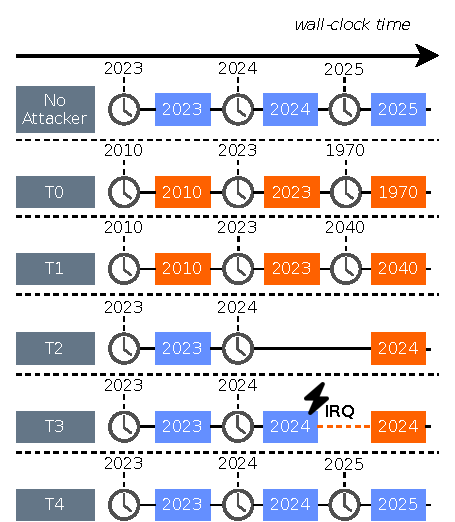
\includegraphics[width=\columnwidth]{figures/time-levels.pdf}
	\caption{Visual representation of different time levels with attacker
	influences marked in orange. \Tzero{} is controlled by the attacker, \Tone can
	only move forward but make jumps, \Ttwo can be arbitrarily delayed, and
	finally in \Tthree the attacker can still interrupt the enclave before it
	utilizes the time. Instead, level \Tfour{} gives the same guarantees as when
	no attacker is present.}
	\label{fig:time-types}
	\vspace{-3ex}
\end{figure}
%\jt{\Cref{fig:time-types}: It's more a visualization of attacker impact.
%Can we highlight the moment the attacker intervenes and maybe make the
%following time box orange?; AEX -> needs to be introduced, or we are more
%general and say "iterruption/exception"?}
%\jo{covered}

\newcolumntype{Y}{>{\centering\arraybackslash}X}
\newcommand{\tableNo}{}
\newcommand{\tableYes}{\faCheck}
\begin{table*}[!t]
	\centering
	\footnotesize
	\caption{
Levels of time and the guarantees given by them. Checkmarks identify that a level protects against this type of attack.
        }
    \begin{tabularx}{\textwidth}{llccccll}    \toprule
        % \bf Type 	& \bf Added guarantee 	& \multicolumn{4}{c}{\bf Attacker controls\dots} & \bf Example time sources &  \bf Discussed use case\\
        % \cmidrule(lr){3-6}
			Type		&	Added guarantee				        & Rollback & Freq. & Delay & Interrupt & Example time source & Discussed use case \\ 
			\midrule
			\Tzero  & None   							          & \tableNo & \tableNo & \tableNo & \tableNo & Untrusted OS    				& ---       \\
			\Tone   & Time monotonically advances   & \tableYes & \tableNo & \tableNo & \tableNo & Untrusted OS \texttt{+} check & Time-based policies        \\
			\Ttwo   & Time moves at constant pace   & \tableYes & \tableYes & \tableNo & \tableNo & ME, timer thread, remote server			& Rate limiting       \\
			\Tthree & Time is read with known delay & \tableYes & \tableYes & \tableYes & \tableNo & Secure TSC, MMIO timer	& Resource counting      \\
			\Tfour  & Use of time is atomic  			  & \tableYes & \tableYes & \tableYes & \tableYes & Trusted scheduler & Credential expiration, DRM       \\
			\bottomrule
		\end{tabularx}
	\label{tab:time-types}
	% \vspace{-2ex}
\end{table*}

This section identifies five successive levels of time tracking approaches for
confidential applications, summarized in \cref{tab:time-types}. These levels are additive, so that each level represents
an increasingly more capable and accurate time source. However, higher levels
may also place more demands on the underlying TEE architecture, and, as
discussed later, lower levels may be sufficient for certain applications.

\Cref{fig:time-types} depicts each time level, together with a sample time trace
reported to and experienced by the enclave. The top row represents the ground
truth, where no attacker is present and wall-clock time advances linearly and at
a constant rate. The running time of the enclave application is visualized in
the colored squares, whereas the clock symbols represent a query to the abstract
time source. The example value returned by the time source is indicated above
the clock symbol and will be used in the subsequent enclave computation, colored
blue if the time is correct w.r.t.\ the wall-clock time, or orange if time is
influenced by the attacker.

%\jt{time level: They are more "approaches to time keeping that come with
%certain temporal guarantees"} \jt{$T_{n}$ looks like elements of a time series
%to me. $Tn$ would be better. Or $An$ for approach?} \jo{not sure, fwiw I think
%\Tone{} etc can also be read as ``timer one'' and then we reason about the
%guarantees such a timer can give..}

\paragraph{\Tzero: No trusted time}
The default case is to have no trusted time, i.e., to fully rely on untrusted
input without performing any checks on the incoming time data. As illustrated in
\cref{fig:time-types}, the observed time can be any point in the past or in the
future and may vary arbitrarily. While this may suffice for testing scenarios,
e.g., annotating untrusted timestamps in a debug log, it is clear that any
application-specific, security-sensitive use of time cannot rely on a \Tzero{}
timer.

\paragraph{\Tone: Monotonically increasing time}
%Trusted monotonic counter from untrusted time source}
If enclaves only have access to an untrusted time source, they can perform
certain minimal checks on received timestamps before acceptance. The most
important check to perform here is to ensure that received time data only ever
increases, i.e., that time never winds backwards. Depending on the granularity
of the untrusted time source and the sampling frequency, additional checks may
be added, e.g., checking that two time queries should never return the same
value or zero. While these checks are minimal and the underlying time source is
still untrusted, the counter value can be stored inside the
enclave and \Tone{} can at least prevent attackers from rewinding  the internal
time of an enclave.
Since \Tone{} timers cannot rely on external data, they have to store the time locally.
This makes them prone to rollback attacks where time is reverted by restarting the enclave with an obsolete local timestamp.
%\Tone may still be utilized to realize a form of monotonic counters where if
%the counter value can be stored securely inside the enclave, the attacker is at
%least never able to rewind the internal time of the enclave. \jt{Isn't it the
%other way around: You need monotonic counters provided by hardware/TEE to
%implement this?} \jo{yes I agree this is confusing and we should avoid using
%the well-established monotonic counters terminology which IMO is strictly
%stronger than \Tone{}}

\cref{fig:time-types} shows that attackers in \Tone{} can advance time at will
and can trigger arbitrarily large time jumps for the enclave.

%\paragraph{\Ttwo: Trusted monotonic counter with fixed frequency}
\paragraph{\Ttwo: Trusted remote time}
To improve time-keeping, the enclave can switch from an untrusted to a remote
trusted time source, guaranteed to have a fixed, known frequency. As such, this
time source can be relied upon for trusted time information, when standard
cryptographic measures are in place to protect and validate the integrity and
authenticity of the time packets over the untrusted network (e.g., this secure
time channel can be configured as part of the attestation protocol). Note that
the ``remote'' trusted time source can be truly remote, e.g., a server reached
over the Internet, but could also be provided on the same system-on-chip, e.g., by a trusted co-processor.
If the monotonicity of the external time source can be trusted, rollback attacks targeting the time value are also not possible anymore since on enclave restarts, the time can be re-queried.
Obviously, rollback attacks are still a threat to enclaves with a \Ttwo{} timer and above, but they will not affect the time stored in the enclave.
%TODO GS: I commented the sentence below because I think it's redundant.
%In both cases, however, the communication channel is
%confidentiality and integrity protected but passes through the untrusted
%operating system.

As the communication channel between the time source and the enclave is still
under the attacker's control in regards to availability, \Ttwo{} time requests
and responses may be arbitrarily delayed. Hence, \Ttwo{} timestamps received by
the enclave can only ever be trusted as a \emph{lower bound} on the reference
wall-clock time. \Cref{fig:time-types} depicts a potential situation where the
attacker would allow the enclave to query the time source, but then delay the
response.

%\paragraph{\Tthree: Trusted monotonic counter with fixed frequency and trusted
%direct channel to time source}
\paragraph{\Tthree: Trusted local time}
In order to prevent arbitrary delay attacks, enclaves must be able to access the
trusted time source through a direct channel without adversary intervention,
e.g., when the time source is an on-chip timestamp counter that can be queried
via dedicated CPU instructions.
%but also be aware of the delay of any communication with the time source. A
%simple solution to know this delay is if the communication channel is secure
%and can be trusted. Another solution would be an atomic operation to directly
%read from a time register that can be trusted.
%
If both time source and channel are trusted, adversaries cannot arbitrarily
delay timestamps anymore before they reach the enclave. This, technically,
grants enclaves access to accurate time information with both a lower and an
\emph{upper bound}.

We argue, however, that in order to utilize such accurate time information in
practice, enclaves also need to be able to act \emph{atomically}, i.e., without
(undetected) attacker-induced interruptions. \Cref{fig:time-types} depicts a
possible attack that is still possible on \Tthree where the adversary precisely
interrupts the enclave right after it reads from the trusted time source. The
adversary can then keep the enclave interrupted until it suits them and only
resume the enclave at a convenient time, effectively reducing the accurate
temporal guarantees back to only the lower bound offered by a \Ttwo time source.

Consider an enclave that only grants access to a resource if
a presented certificate is valid, and denies access otherwise. If the
adversary begins the validation process at a time that the certificate is still
valid, the enclave will read a permissible time from the time source. Right
after the time value has been read into the enclave, the adversary could however
interrupt the enclave. % for an arbitrarily long time. 
When the enclave is later resumed, the adversary could gain access to the resource even if the initially
presented certificate is not valid anymore.

\paragraph{\Tfour: Trusted and atomic local time}
% \jt{I feel that this this requires
% design decisions that someone who is aware of TOCTOU attacks would avoid. It's
% gonna be confusing for reviewers to have atomic processing and still get
% interrupted.}
% \jo{not sure I follow; you mean this is ultimately application-specific?}
% \jt{resolved.}

The dangers of the above attack vector are nuanced. Many interruption attacks on
\Tthree timers only work if the adversary initially had access to a resource.% in the first place. 
Thus, arguably, maintaining this access until after the
credentials expired can be considered as a parallel issue to denial of service
attacks where output of the enclave is delayed by the adversary. We note,
however, that for some applications and use cases this attack vector may not be
acceptable and enclaves should only present an output at the correct time. We
discuss two examples of this in \cref{sec:usecases:tfour}.

% An intuitive addition to certificate checking would be the case of
% \ac{DRM} where such certificates may be given to renters
% of movies who should lose access to rented resources after a given time has
% passed. Similarly, holders of short lived certificates may only ever be allowed
% to access old information but never information after their certificates
% expired. If enclaves cannot be trusted to atomically check and then act upon a
% time source, adversaries may be able to present outdated time and certificate
% information to retrieve new data.

% Only if an enclave can utilize the trusted time source via a trusted channel
% without experiencing interrupts can the enclave reliable make use of trusted
% time. The reasoning behind this is evident when discussing the use case of
% certificate checking given in \cref{tab:time-types}. 

% \begin{enumerate}[label=R\arabic*]
% 	\item \label{req:tts} \emph{Trusted Time Source (TTS):} the
% 	most basic requirement. This means that the time source works as intended,
% 	i.e., time advances correctly and attackers cannot tamper with it. The TTS
% 	can be either in the same physical node as the enclave or external;
% 	\item \label{req:channel} \emph{Secure channel:} if the channel
% 	is not protected wrt. integrity and authenticity, attackers in the network
% 	or in the OS can easily tamper with the time information;
% 	\item \label{req:delay} \emph{Predictable or
% 	attacker-independent delay:} The enclave should be able to measure the
% 	transmission time of a time value sent from the TTS to the enclave, or it
% 	should happen within a fixed upper bound;
% 	\item \label{req:irq} \emph{Interruption protection:} To
% 	prevent TOCTOU attacks, the enclave should not be interrupted  by the
% 	OS/hypervisor while processing the time information, or at least it should
% 	be able to \emph{detect} interruptions.
% \end{enumerate}

% Reqs.~\ref{req:tts}-\ref{req:channel} enable a Lower Bound on the elapsed time,
% because the enclave has always the guarantee that, for each value $t$ produced
% by the TTS, the enclave will receive $t$ at a time $t^\prime = t + \triangle t$,
% where $\triangle t \geq 0$. Here, $t_{LB}$ is always equal to the most recent
% $t$ received by the enclave. Additionally, if the TTS is synchronized with the
% \ac{UTC}, the enclave obtains a LB on absolute time.

% To enable an Upper Bound on elapsed time, it is essential to allow the enclave
% accounting for any delays that incur from when a time value is sent by the TTS
% to when the value is actually used inside the enclave, thus requiring all
% Reqs.~\ref{req:tts}-\ref{req:irq}. Indeed, arbitrary and non-measurable delays
% or undetected interruptions during that time would make it impossible for the
% enclave to estimate $\triangle t$ in order to compute $t^\prime$.

% In practice, Req.~\ref{req:delay} can be satisfied by a local TTS that the
% enclave would be able to access without incurring a context switch. Having the
% TTS in the same node as the enclave is essential to deal with unpredictable
% network delays, while the absence of context switches to access it is needed to
% ensure that the OS/hypervisor does not delay resuming the enclave indefinitely.
% Instead, Req.~\ref{req:irq} can be satisfied by the ability to detect an
% interruption, such that the enclave does not trust any time values received
% before the interruption because the OS/hypervisor may interrupt the enclave
% indefinitely. Note that the enclave should distrust any time values received
% before performing an OCALL, for the same reason.

% The aforementioned requirements ensure either that the enclave is able to
% compute an UB, or that the enclave detects an interruption and needs to try
% again. In both cases the enclave is protected from malicious activity.
% Additional requirements such as non-interruption may give enhanced benefits,
% but are considered optional.


% For all synchronizations of time, there is a delta between the actual time and
% the time that the client, in this case the enclave, knows. This time delta is
% defined as $\triangle t = t_{actual} - t_{enclave}$.

% Core assumption: Even with a trusted setup phase that eliminates any attacker
% effect on the network overhead (and as such makes the NTP time synchronization
% near perfect), there are still three types of time:

% \begin{description}
% 	\item[\textbf{T1: Logical clock as a proxy for time}:] ROTE, Lamport clocks but also time epochs. $\triangle t$ is unknown and irrelevant.
% 	\item[\textbf{T2: Lower time bound on elapsed time}:] enclaves, distributed systems. $\triangle t$ is again not known.
% 	\item[\textbf{T3: Upper time bound on elapsed time}:] Here, $\triangle t$ must be known.
% \end{description}

\section{Intel SGX}
\label{arch:sgx}

The Intel SGX architecture does, in itself, not provide any notion of trusted
time. However, several proposals exist to provide trusted time services to SGX
enclaves.

%\subsection{Time Sources}

\paragraph{Platform service}
Intel provides \ac{PSW} to set up and use trusted time and monotonic
counters~\cite{cen2017trusted}. Particularly, the PSW offers a \Ttwo{} time
source based on a coarse-grained clock in the Intel \ac{ME}, a chip that
physically resides on the same package but is entirely separate from the main
CPU. This allows timer-based policy enforcements on offline platforms that are
not necessarily connect to a network. All communication between enclaves and the
\ac{ME} passes via the untrusted operating system and is, hence,
cryptographically protected, but can be arbitrarily delayed. Enclaves can use
the \texttt{sgx\_get\_trusted\_time} API to track the amount of time (in
seconds) passed since a previous read of the timer.
%
ME services are excluded in the Intel SGX Linux PSW from version 2.8 from 2020
onwards.
% and it is now no longer possible to get either functionality from the PSW.

% from whitepaper: Trusted time – for timer-based policy enforcement on offline
%platforms that don’t have access to remote time servers for trusted calendar
%time. Monotonic counter – for replay protection of offline storage, enforcement
%of counter-based policies, etc
%
% track the amount of time passed since a previous read of the timer no wct,
% coarse-grained, real-time clock

% time-based policy DRM sample code
% crypto-protected channel session

% Discuss external TTS (e.g., TPM, or a remote server).

\paragraph{Timestamp counter}
Initial SGX versions did not allow to execute the x86 \inst{RDTSC} instruction
to receive the processor's internal \ac{TSC} in enclaves. However, more recent
SGX2 processors now support the \inst{RDTSC} instruction in enclave mode,
with an explicit warning that the instruction may be trapped and the
timestamp returned may be influenced by the untrusted operating system.

% Discuss the RDTSC/RDTSCP support in SGX2 (and related WRMSR).
%\texttt{CR4.TSD}%
% effectively a \Tzero{} timer
% explicit disclaimer in intel sdm

We experimentally confirmed that privileged adversaries can arbitrarily control
the values returned by \inst{rdtsc} on SGX2 platforms by directly manipulating
the underlying \texttt{IA32\_TIME\_STAMP\_COUNTER} \ac{MSR}. For this, we
developed a sample enclave that executes two \texttt{rdtsc} instructions and
returns the measured cycle difference. One would expect this difference to
always be positive and reflect the elapsed time in between the two \inst{rdtsc}
instructions. However, in our proof-of-concept, we make the observed time in the
enclave move ``backwards'' by interrupting the enclave and overwriting the
\ac{TSC} value using the privileged \inst{wrmsr} instruction in between both
\inst{rdtsc} calls. Thus, we conclude that \inst{rdtsc} on current SGX platforms
is not any better than an adversary-controlled \Tzero{} timer.

We note, however, that the \ac{TSC} \ac{MSR} is duplicated per logical processor
and can, hence, only be changed by interrupting the enclave. That is, as long as
the enclave is not interrupted, any successive \inst{rdtsc} reads will behave as
a trusted \Tfour{} timer that monotonically increases at fixed frequency. This
may be leveraged with upcoming ISA changes~\cite{intel2022aexnotify} that will
make SGX enclaves interrupt-aware. 
At the same time, the restriction that an enclave is never interrupted may be
too limiting for some real-world deployments.

\paragraph{Academic timers}

TrustedClock~\cite{jigsaw} is a system that relies on an interrupt handler in
\ac{SMM} to implement functionality that is similar in its security guarantees
to \texttt{sgx\_get\_trusted\_time} by the Intel SGX \ac{PSW}. The authors base
their security argument on the handler being loaded at boot time with a secret
key that is not accessible at runtime by the untrusted OS. Enclaves can then
communicate with the handler by establishing a secure channel based on the
pre-shared public key. Aside from the security implications of including the
unattested SMM handler in the trusted computing base,
% loading and storing such a security sensitive piece of code that contains a secret on the same system as the untrusted OS, 
TrustedClock is stated to not be completely immune to timer modifications by the untrusted OS.
Instead, TrustedClock relies on combining several x86 hardware timers
and asserting their monotonicity (similar to \Tone{}), thus
making it harder for a malicious OS to precisely tamper with all involved
timers at the same time.
%validate the credibility of time value
%rely on all timers available on x86 which are not necessarily all protected 
%While TrustedClock may thus make it harder for a malicious OS to precisely tamper with all involved
%timers at the same time, the attack vector is not eliminated completely. 
%Lastly, TrustedClock requires the enclaves to have knowledge of the public key
%inside the SMM at compile time which is unrealistic for large scale
%deployments.

TimeSeal~\cite{anwar2019securing} utilizes a cohort of multiple threads that
each periodically poll \texttt{sgx\_get\_trusted\_time} to monotonically
increase the time. The authors argue that by using multiple threads and nuanced
synchronization policies between the threads, attacks can be limited in their
scope. Nonetheless, attackers that delay or prevent scheduling of timer threads
at convenient times, such as right before a thread returns a time response, will
be able to skew the reported time of TimeSeal. Additionally, with the
discontinuation of \texttt{sgx\_get\_trusted\_time} on Linux systems, TimeSeal
may not be implementable anymore as of today.

%\newcommand{\xrot}[1]{\hspace{-.4em}\rotatebox{20}{\footnotesize#1}\hspace{-.4em}}
\newcommand{\xrot}[1]{#1}
\newcommand{\xtwo}{\Ttwo{}}
\newcommand{\xone}{\Tone{}}
\newcommand{\xzero}{\Tzero{}}
\newcommand{\xpoc}{\Tzero{}*}
\newcommand{\xna}{--}
\newcommand{\xcat}[2]{\multirow{#1}{*}{\rotatebox{90}{\footnotesize\textsl{#2}}}}
\begin{table}[t]
  \small
  \vspace{-1ex}
  \centering
  \caption{Intel SGX software projects and their use of time. Stars indicate that we prototyped a proof of concept to roll back time for a project. Intel SDK is shown for Linux/Win.
    }
  \vspace{-2ex}
  \label{tab:sgx-overview}
  \adjustbox{max width=\linewidth}{
  \setlength\tabcolsep{3pt}  
  \begin{tabular}{ccccccccc}
  \toprule
  \xrot{SDK} & \xrot{OE} & \xrot{EDP} & \xrot{Gramine} & \xrot{LKL} & \xrot{Occlum} & \xrot{Mystikos} & \xrot{Ego} & \xrot{Enarx} \\
  \midrule
  \href{https://github.com/intel/linux-sgx/releases/tag/sgx_2.8}{---}/\href{https://cdrdv2-public.intel.com/671508/sgx-sdk-developer-reference-for-windows-os.pdf}{\xtwo} & 
  \href{https://github.com/openenclave/openenclave/blob/cd72fd7069488ba6f453c8f5f47bd9fd9a6e6c0d/enclave/core/time.c#L8}{\xpoc} & 
  \href{https://github.com/fortanix/rust-sgx/blob/a7ee253352856b35e54be22c505775c6556ffa82/intel-sgx/enclave-runner/src/usercalls/mod.rs#L1555}{\xzero} & 
  \href{https://github.com/gramineproject/gramine/issues/595}{\xone} & 
  \href{https://github.com/lsds/sgx-lkl/blob/b6e838e0034de86b48470b6a6bf87d2e262e65c9/src/enclave/enclave_timer.c#L29}{\xone} & 
  \href{https://github.com/occlum/occlum/blob/500ca21d527f700d458df10b891948627f396d97/src/libos/src/time/mod.rs#L76}{\xpoc} & 
  \href{https://github.com/deislabs/mystikos/blob/7ce616416a310aabb543517ed3a9625c1f4acb70/kernel/itimer.c#L32}{\xzero} & 
  \href{https://github.com/edgelesssys/edgelessrt/blob/9191ff25a0424d21a22c85eb12b09ebe5f407c3f/src/ertlibc/time.cpp#L53}{\xone} & 
  \href{https://github.com/enarx/enarx/blob/4c1d3db4039e1f2af4b251a202e64a2cdc0729fb/crates/sallyport/src/guest/call/syscall/clock_gettime.rs#L16}{\xzero} \\
  \bottomrule
\end{tabular}
}
% \vspace{-2ex}
\end{table}

%\subsection{Software Ecosystem}
\paragraph{Software ecosystem}
Several shielding systems offer a ``lift-and-shift'' approach to port legacy
applications to SGX. However, these applications were not designed for SGX's
threat model and may rely on sane OS time services.

\Cref{tab:sgx-overview} summarizes how existing SGX shielding systems expose the
untrusted OS time to applications. Interestingly, we found that most projects
include a warning, but forward OS time without any restrictions (\Tzero{}),
whereas the Gramine and LKL library operating systems at least ensure that time
does not move backwards (\Tone{}). We developed two minimal proof-of-concepts to
demonstrate backwards time advances in OpenEnclave and Occlum. We, hence,
recommend that all projects include minimal checks to adopt the \Tone{} time
model.

%Many projects expose the untrusted OS time to applications without any warnings/restrictions.
%Software engineers that leverage such projects without expertise on TEEs might not even realize that their applications might suffer from such vulnerabilities.


% \section{Discussion and other TEEs}

% Possible options:
% \begin{enumerate}
% 	\item reduce trust assumptions
% 	\item allow breach and only detect time issues post-compromise
%  	\item atomicity after checking time
% \end{enumerate}


%\section{Architectures}
% \label{sec:architectures}

% \newcommand{\rot}[1]{\rotatebox{0}{#1}}
% \newcommand{\yes}{\faCircle}
% \newcommand{\no}{\faCircleO}
% \newcommand{\maybe}{\faAdjust}
% \newcommand{\unknown}{\faQuestion}
% \begin{table*}[!t]
% 	\centering
% 	\footnotesize
% 	\caption{}
% 	\resizebox{\linewidth}{!}{
% 		\begin{tabular}{|l|cccc|ccc|}    \toprule
% 			\rot{Architecture} & \rot{\ref{req:tts}} & \rot{\ref{req:channel}} & \rot{\ref{req:delay}} & \rot{\ref{req:irq}} & \rot{Enclave time} & \rot{LB elapsed time} & \rot{UB elapsed time} \\ 
% 			\midrule
% 			Intel SGX 	  	   & \maybe   & \yes       & \no        & \yes       & \no        & \yes       & \no       \\
% 			Intel TDX		   & \maybe   & \yes       & \no        & \yes       & \no        & \yes       & \no       \\
% 			AMD SEV			   & \unknown & \yes       & \no        & \unknown   & \unknown   & \yes       & \no       \\
% 			ARM TrustZone	   & \yes     & \yes       & \yes       & \yes       & \yes       & \yes       & \yes      \\
% 			TPM				   & \maybe   & \yes       & \yes       & \yes       & \no        & \no        & \no       \\
% 			\bottomrule
% 		\end{tabular}
% 	}
% 	\label{tab:architectures}
% \end{table*}

\section{Other Architectures}
\paragraph{Intel TDX}

The TDX specification~\cite{intelTdxSpec} discusses \ac{TSC} virtualization,
which provides a consistent virtual \ac{TSC} value to a \ac{TD} among all its
vCPUs. The virtual \ac{TSC} starts counting from zero when the \ac{TD} is
initialized and runs at a fixed frequency defined by a parameter stored in the
TD configuration. Guest \acp{TD} can access the virtual \ac{TSC} using the
\inst{RDTSC} instructions, and its value is calculated from the physical
\ac{TSC} adjusted to the \ac{TD}'s offset and frequency. 

We analyzed the source code of the TDX module, which makes sure that the
\ac{TSC} is not modified before a \ac{TD} enter
%
%while the TD is not running by comparing the \texttt{TSC\_ADJUST} \ac{MSR} , which
%is used to synchronize the \ac{TSC} across multiple logical processors in the
%Intel architecture~\cite{intelManual}. Whenever the TSC is modified via the
%\inst{WRMSR} instruction, the \texttt{TSC\_ADJUST} value is updated as well.
%This enables \ac{TSC} tampering detection 
%
by comparing the current \texttt{TSC\_ADJUST} \ac{MSR} value against a reference
value stored on \ac{TD} creation, raising an exception if a mismatch between the
two values occurs.
%
% The TDX module stores the value of \texttt{TSC\_ADJUST} in secure memory at TD
% boot time and raises an exception if the register has been modified before
% \inst{TDENTER}. 
%
This allows \acp{TD} to obtain a stable and consistent \ac{TSC} value across
\ac{TD} lifetime, guaranteeing a time level \Tthree{}.

\paragraph{AMD SEV}

The AMD SEV-SNP~\cite{AmdSevSnp} extensions introduced a so-called \emph{Secure
\ac{TSC}} feature, which should provide enhanced protection against \ac{TSC}
manipulations. The Secure \ac{TSC} feature can be enabled by a guest VM at boot
and prevents the hypervisor from intercepting any \inst{RDTSC} instructions
called by the guest VM. Furthermore, the calculation of the \ac{TSC} value is
made using offset and frequency parameters stored in VM secure memory, thus not
accessible by a malicious hypervisor. However, it is unclear from the
specification whether the Secure \ac{TSC} feature prevents the hypervisor from
directly writing into the \ac{TSC} via the \inst{wrmsr} instruction, similar to
our proof-of-concept on SGX2. In such case, the hypervisor could effectively
tamper with the \ac{TSC} while the guest VM is not running, preventing it from
leveraging a stable and consistent representation of elapsed time. Without such
guarantee, the \ac{TSC} counter would only be a \Tzero time level for SEV-SNP
guest VMs.

\paragraph{ARM TrustZone}

ARM TrustZone~\cite{pinto2019demystifyingtz} separates progam execution into two
protection domains, the secure world and the normal world. Both worlds are
hardware-isolated, run their own OS, and normal-world software is prevented from
directly accessing secure world resources. TrustZone also allows for system
devices, such as a time source, to be restricted to one world. This, however, is
implementation specific, with the TrustZone protection controller being
an optional component. TrustZone further extends the processor's interrupt
controller with prioritized secure and non-secure interrupt sources to prevent
denial-of-service attacks from the normal world. Based on these features, ARM
TrustZone supports up to \Tfour{}, and has been previously leveraged to
implement secure real-time systems~\cite{wang2022rttee} or TPM functionality in
software~\cite{raj2016ftpm}.

\paragraph{ARM CCA}
ARM confidential compute architecture~\cite{arm-cca} adds additional execution
worlds to the ARM architecture that allow to run multiple so-called Realms in
parallel to the ARM TrustZone secure world. All Realms are all managed by a
trusted realm management monitor (RMM) component~\cite{arm-rmm}. While each
Realm has direct access to architectural timers, the RMM does not make
scheduling decisions or manage interrupts, both controlled by the untrusted
hypervisor~\cite{arm-cca}. As such, ARM CCA has access to a \Tthree{} time
source.

\paragraph{TPM}

A \ac{TPM} is a hardware-based security component that provides a secure foundation
for system integrity usually in form of a co-processor.
% , such as the integrity measure
% architecture~\cite{sailer2004design}, and cryptographic operations, such as
% direct anonymous attestation~\cite{brickell2004direct}.
\acp{TPM} comprise timing components and monotonic counters. According to the
specification~\cite{TPM2.0-Rev-01.59}, a \ac{TPM} includes two primary timing
components referred to as \emph{Time} and \emph{Clock}. The \emph{Time}
component is separate hardware that provides the number of milliseconds since it
has been powered on and cannot be controlled by software. The \emph{Clock}
component yields a value that software can advance but can never roll back. 
% The \emph{Clock} value can be adjusted by external software via the functions \texttt{TPM2\_ClockSet()} and \texttt{TPM2\_ClockRateAdjust()}.
% However, authorization from the platform or owner is required for both actions.
% This means that an adversary cannot call these functions arbitrarily without proper authorization. 
% Nonetheless, if an attacker has control over the untrusted environment, they can intercept and modify the requests sent to the TPM, thereby taking control of the \emph{Clock} value.
%
%Thus, the \ac{TPM} can leverage its \emph{Time} component for accurate
%measurements of elapsed time. The \emph{Clock} component can be used to align
%the internal time value to an external reference such as the \ac{UTC} time, although
%an adversary that has control over the platform can advance the \emph{Clock}
%value as much as they want. 
%

Thus, by mapping this specification to our time levels, the \emph{Clock}
component only guarantees a \Tone{} time, since a privileged adversary can
advance the \emph{Clock} value arbitrarily, while \emph{Time} may reach up to
the \Tfour{} level if an offset is securely provided to the \ac{TPM} to align
its value to the wall-clock time. However, according to~\cite{TPM2.0-Rev-01.59},
attackers may change the \ac{TPM} clock frequency by at most $\pm{}32.5\%$,
which should be taken into account when checking the time.

% Removed for space
% \subsection{Embedded TEE}
% \todo{todo: eithr do a summary here or focus on Aion?}

\section{Use Cases}

This section focuses on use cases that rely on some form of time. To facilitate
this discussion, we adopt an incremental approach, beginning with time-based
policies that only necessitates level \Tone, and gradually progressing through
each level up to credential expiration, which requires \Tfour.

\subsection{Time-Based Policies}
A simple time-based policy is that a user that once lost access to a
resource will not regain access to it. By utilizing \Tone, enclaves
can enforce this behavior so that the attacker cannot revert time to
regain access. Enclaves can be useful in systems where the OS is initially in a trusted
state but may become compromised during runtime. In this case, the enclave would periodically be invoked with linearly increasing timestamps and then at some time be invoked with an old timestamp.
If the attacker timestamp precedes the last timestamp sent by the benign operating system, the 
enclave would be able to detect this attack and prevent access.

It is important to note that, by using \Tone, the enclave will not be able to
revoke access if the OS does not wish this to happen, as progress of time is
still attacker-controlled. 
The only guarantee is that, once revoked, access can
not be reinstated. This is similar to \emph{Clock} guarantees of \acp{TPM}~\cite{TPM2.0-Rev-01.59}.
Similarly, using \Tone timers assumes that rollback attacks on the enclave state can be detected by the enclave. Otherwise, the adversary could restart the enclave and provide a stale timestamp or stale sealed data to the restarted enclave to get the desired result.
If rollback attacks on the time value can not properly be prevented, a \Ttwo timer has to be used.% to secure time-based policies.
%  and is being utilized by various projects such as the Mirosoft Confidential
%  Computing
%  Framework~\footnote{\url{https://github.com/microsoft/CCF/pull/4786}}.

% not regaining after  you already revoked (eg later adversarial takeover)

% One of the most basic requirements for enclave applications is that of state
% continuity, i.e., that enclave state can not be rolled back but only move
% forward. This can be realized with a simple \Tone clock that can only ever
% increase. If this state should also persist across enclave restarts, the state
% variable must stay consistent during enclave shutdowns so that the untrusted OS
% can not roll back the enclave state. Distributed logical clocks over a network
% can solve this challenge by employing a network of enclaves that ensure this
% monotonicity~\cite{matetic2017rote}.

\subsection{Rate Limiting and TOTP}

\subsubsection*{Rate Limiting}
%
Time-based rate limiting is a mechanism often used to narrow the impact of brute
force attacks. Consider a service running in an enclave that performs password
checking~\cite{krawiecka2018safekeeper}. If time is OS-controlled, time-based
rate limiting would not be effective as attackers can artificially advance time. The service would easily be tricked into processing more
requests than desired. Thus, \Tone{} is not a sufficient time level
for rate limiting. Only when the frequency of the clock is independent from the
attacker can the enclave rely that at least a minimum amount of time has passed.

This use case does not have higher requirements on the time
source than a \Ttwo time source. It does not matter
whether a minute or a year has passed between two requests as long as \textit{at
least} a minimum amount of time has passed. If the
untrusted OS increases the time between requests, this does not go against the
security guarantees offered by rate limiting and would only impact
availability of the service.

% While slowing time might cause similar issues as explained before, such as
% guessing a OTP, accelerating time might enable, instead:
% \begin{itemize}
% 	\item sending tons of requests in a short time (DoS)
% 	\item brute-force attacks on regular passwords/PIN codes.
% \end{itemize}

\subsubsection*{TOTP}
%
\Acp{TOTP}~\cite{rfc6238} are commonly used in second-factor
authentication systems. The algorithm takes as input a fixed parameter $k$ (e.g., a
key) and a variable parameter $x$, and gives as output the one-time password,
which is simply computed as a HMAC truncated to the desired size. In \ac{TOTP},
the variable parameter $x$ depends on the current time $t$, an initial value
$t_0$, and a fixed time window $W$ according to the equation $x = \left\lfloor(t
- t_0)/W\right\rfloor$. Typically, $x_0$ is equal to 0 and $W$ is equal to 30
seconds. This means that, within the same 30-second window, the resulting OTP
will always be the same, provided that the same \emph{k} is given as input. As
such, attackers who have control over the time source, as in levels \Tzero and
\Tone, could potentially slow down or even freeze the time perceived by the
\ac{TOTP} server, preventing the OTP from changing. This could be exploited by
attackers to circumvent the second factor authentication provided by \ac{TOTP},
either through brute-force attacks or by reusing an old OTP previously used by
the legitimate user. Thus, we conclude that \ac{TOTP} %similar to rate limiting
requires a \Ttwo time source.

In the context of Intel SGX, a few projects have proposed the use of \ac{TOTP} authentication.
For instance, SGX-UAM~\cite{wu2021sgx} utilizes \ac{TOTP} to authenticate a
client to the identity provider, while SCONE~\cite{scone2fa} employs it as
a second-factor authentication for their configuration and attestation server.
While the former utilizes \texttt{sgx\_get\_trusted\_time}, now
discontinued on Linux, it is unclear which time source is used by the latter.

\subsection{Resource Accounting}

When utilizing confidential computing in cloud environments, both users and
cloud providers may require a trustworthy and accountable measurement of spent
resources during a computation. Interesting nuances with this use case occur
when code running inside the enclave is not necessarily trusted by both parties
that wish to rely on the measurement.
% \christoph{is the code running in the enclave ever trusted by the cloud provider? I feel this is missing the point a bit, it's the trust in time that is of interest}
% FA: Yes, I kind of agree but at the same time it's easy to forget that internal counting is not enough since the cloud provider doesn't trust this. Jo ran into this multiple times so I'd rather be explicit about it.
Take for example the case of
Function-as-a-Service in enclaves~\cite{sfaas}. There, workload providers run a workload and only wish pay for the resources used. If possible, workload providers may want to pay less than what they owe. Cloud providers, on the other hand, may wish to overestimate the
resources consumed and demand more compensation.

The cloud provider can always make accurate estimates on enclave time, since the
workload runs on their infrastructure. However, the workload provider cannot
trust any time levels below \Tthree{}:
If the untrusted OS controls the time, such as in \Tzero or \Tone, 
time can be manipulated to overestimate resource consumption, leading to higher billing for the workload provider. 
Furthermore, even with a \Ttwo clock the cloud provider could arbitrarily delay the enclave communication with the clock and artificially increase the workload time. 
Only if the channel to
the clock is independent from the cloud provider, and the clock is independent
from influence, the time source can be accurately utilized for resource
accounting. Note that, without a full \Tfour utilization of the clock, the cloud
provider could still cheat and interrupt the workload for periods of time. In
this case, the system would need to be set up in a way that punishes such
behavior and undercounts time spent potentially interrupted, e.g., through means
of resetting the count on interrupt reentries.

\subsection{Credential Expiration and DRM}
\label{sec:usecases:tfour}
%
A common use cases for using time is to check the validity of
credentials, such as PKI certificates and \acp{JWT}. Typically, these
credentials have a validity window defined by a \emph{Not Before} and a
\emph{Not After} field. Thus, it is important that the time source provides a
reliable time to correctly validate such credentials, e.g., during the
TLS-handshake or the authorization step at application level.

If time is not reliable inside the enclave, it could lead to security breaches
such as allowing access to sensitive data to unauthorized users.
%  (e.g., an employee that has left the company).
If an untrusted \Tzero{} or \Tone{} clock is used, attackers may rewind the time perceived by the enclave to fall within the validit window of an expired certificate.
% Attackers may manipulate the time perceived
% by the enclave to fall within the validity window of a certificate by exploiting
% untrusted time sources such as \Tzero{} and \Tone{} clocks, either through
% direct tampering of the time information or by altering the clock frequency of
% the time source. 
If instead stronger \Ttwo{} or \Tthree{} timers are used, the adversary may still induce network delays and/or interrupts to coerce the enclave into accepting credentials that were valid at the beginning of the communication, but have expired before their actual use. 
This problem is exacerbated when credentials are short-lived: typically, access
tokens are refreshed frequently and thus have a rather short lifetime of minutes
to hours~\cite{rfc6819}. Thus, the enclave should only trust a time level
\Tfour{} in order to make correct decisions.
%
%Instead of relying on trusted time, another potential solution to this issue
%involves implementing an appropriate revocation mechanism. While the revocation
%of JWTs remains an unresolved challenge~\cite{janoky2018analysis}, Certificate
%Revocation Lists (CRLs) are typically used for PKI certificates. However, it is
%often unfeasible to add every expired certificate to a CRL, due to the
%significant size and management difficulties of the resulting list. Indeed, in
%practice non-compromised certificates are typically excluded from the CRL, while
%compromised certificates are removed from the list upon
%expiration~\cite{rfc5280}. Thus, CRLs might create a false sense of security
%when a reliable time source is not available. A more promising approach to check
%the validity of a credential in enclaves could be relying on an online check
%against a trusted remote server, such as in OCSP stapling~\cite{rfc6961}.

The open-source \texttt{rust-mbedtls} library written by
Fortanix~\cite{rustMbedtls} allows TLS-termination inside SGX enclaves.
Time-validity of certificates is only checked if the \texttt{time} feature is
enabled, which means that either it is not checked at all (if disabled), or it
is checked against the insecure OS time (if enabled). This shows that the
absence of a trusted time source in SGX can potentially compromise the security
of applications, thus software engineers should take into account such
limitations when developing their applications.
%Furthermore, CRLs must be
%manually provided, and regularly updated, by the application. Under these
%circumstances, it is non-trivial to secure network connections properly,
%especially when software engineers are unaware of such limitations.
%

The use case for DRM can be reduced to an instance of credential expiration,
where a user wants to access a resource that should already be locked to them.
If the enclave is interrupted after the authorization check but before the use
of the resource, the latter might take place when the user has no longer
permission to access it.

% \subsection{Something with guaranteed \& timely sensing or actuation?}
% \todo{idea}

% \subsection{DRM Time-Based Policy} \todo[inline]{FA: I referenced this one
% already in t4 when explaining that, so write this with a pointer back} eg SGX
% rental period?
% https://download.01.org/intel-sgx/linux-1.8/docs/Intel_SGX_SDK_Developer_Reference_Linux_1.8_Open_Source.pdf



% \section{Related Work}

% \paragraph{On Monotonic Counters:}

% \cite{sarmenta2006counters, cen2017trusted, lee2019tzlogs, martin2021counters}


\section{Conclusions}
Tracking the passage of time is nuanced when relying solely on measurements that
are partially controlled by an adversary. To better reason about the usage of
time inside TEEs, we identified five progressive levels of time-keeping, \Tzero
to \Tfour and classified the popular Intel SGX as well as other commonly used
TEEs. Considering relevant use cases such as rate limiting or resource counting,
we show that not every application requires access to the highest level of time,
for which existing solutions may already suffice. However, this classification
also shows that other use cases, such as credential expiration, need stronger
time guarantees that most architectures cannot yet provide. Thus, reliable
time-keeping is highly application-specific and software engineers should take
into account the limitations of current technologies.

%%
%% The acknowledgments section is defined using the "acks" environment
%% (and NOT an unnumbered section). This ensures the proper
%% identification of the section in the article metadata, and the
%% consistent spelling of the heading.
\begin{acks}
This research is partially funded by the Research Fund KU Leuven, by the
Flemish Research Programme Cybersecurity, and by the CyberExcellence
programme of the Walloon Region, Belgium. This research has received funding
under EU H2020 MSCA-ITN action 5GhOSTS, grant agreement no. 814035. Fritz Alder
and Jo Van Bulck are supported by a grant of the Research Foundation -- Flanders
(FWO).
\end{acks}

%%
%% The next two lines define the bibliography style to be used, and
%% the bibliography file.
\bibliographystyle{ACM-Reference-Format}
\bibliography{paper}


%%
%% If your work has an appendix, this is the place to put it.
% \appendix


\end{document}
\endinput
%%
%% End of file `sample-sigconf.tex'.
